%% Marco Teórico C1 %%

\chapter{Paradigmas}

``Las herramientas que utilizamos tienen una profunda (¡y retorcida!) influencia en nuestros hábitos de pensamiento, y, por lo tanto, en nuestra habilidad mental'', Edsger Dijkstra. \\

Los paradigmas de programación guían la forma en que debe construirse una solución para resolver problemas utilizando herramientas computacionales. Cada paradigma tiene sus ventajas y desventajas de acuerdo al tipo de problema que se deseé resolver. En este capítulo se revisan las dos principales corriente \emph{imperativa} y \emph{funcional}, soportadas en las \emph{Máquinas de Turing} y el \emph{Cálculo Lambda}, respectivamente.

\section{Modelo computacional}

Para el estudio de la \emph{computación} desde un enfoque teórico, es necesario utilizar abstracciones que cumplan con las siguientes restricciones:

\begin{enumerate}
	\item El modelo debe ser lo suficientemente poderoso para poder realizar cualquier método computacional físicamente realizable. Sólo de esta forma se puede garantizar que los resultados encontrados puedan ser aplicados en cualquier \emph{Computador Universal} (aquellos que pueden realizar todos las operaciones conocidas sobre una entrada discreta).
	\item El modelo debe ser lo suficientemente simple para facilitar los análisis y las demostraciones a realizar, siendo menester que dicha abstracción elimine detalles innecesarios, cómo por ejemplo, las especificaciones propias de la máquina o las restricciones de un lenguaje de programación específico.
\end{enumerate}  

En ese órden de ideas, han surgido múltiples abstracciones que si bien, han inspirado caminos diferentes para la solución de problemas, han resultado siendo equivalentes en poder computacional; es decir, que en los modelos que se exponen a continuación, aplican los mismos principios de la \emph{teoría computacional}, así como también tienen los mismos límites en cuánto a \emph{computabilidad} se refiere.

\subsection{Máquina de Turing}

``(Turing)ha tenido éxito por primera vez en encontrar una definición absoluta de una interesante noción epistemológica, por ejemplo, una que no depende del formalismo seleccionado'', Kurt Gödel. \\

La Máquina de Turing (TM, por sus siglas en inglés), desarrollada por el matemático Alan Turing, ha servido como el principal modelo bajo el cuál se han construido las computadoras modernas.

\begin{defn}[Definición formal de una TM]\end{defn}

Formalmente, una TM $M$ está descrita por una tupla $(\Gamma, Q, \delta)$  \cite{Arora2009}, que contiene:

\begin{itemize}
\item Un conjunto finito $\Gamma$ de símbolos que las cintas de $M$ pueden contener. Usualmente se tienen 3 cintas, una de entrada, una de trabajo y una de salida, y sobre estas la máquina realiza las operaciones necesarias. Se asume que $\Gamma$ tiene un símbolo ``blank'', denotado por $\Box$; un símbolo ``start'', denotado por $\rhd$; y los número 0 y 1|. Llamamos $\Gamma$ el \emph{alfabeto} de $M$.

\item Un conjunto finito $Q$ de los posibles estados en los que el registro de $M$ puede encontrarse. Asumimos que $Q$ contiene designado un estado inicial, denotado por $q_{start}$, y un estado de terminación (\emph{halting}), denotado por $q_{halt}$.

\item Una función $\delta$: $Q \times \Gamma^k \to Q \times \Gamma^{k-1} \times \{L,S,R\}^k$, donde $k \geq 2$ y $L$: left. $S$: stay. $R$: right., describiendo las reglas que $M$ usa para realizar cada paso. Esta función es llamada \emph{función de transición} de $M$. 
\end{itemize}

Una máquina de Turing es un computador moderno simplificado. Cualquier algoritmo puede traducirse en un conjunto de reglas y símbolos, de forma que pueda ser simulado por una TM.

\begin{figure}
	\centering
	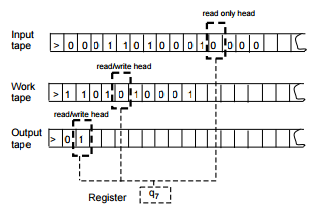
\includegraphics{images/tm}
	\caption{TM con 3 cintas.}
\end{figure}

\subsection{Cálculo Lambda}

El cálculo lambda $\Lambda$ creado por Alonso Church en los 30 para dar una teoría general de las funciones \cite{Bar1998}. Tiene por objeto formalizar el empleo de funciones como transformación de argumentos en resultados empleando un conjunto de axiomas, y reglas de inferencia.

\subsubsection{Sintaxis}

Dado un conjunto \texttt{A} de nombres de variables tal que $\vert$ 
\texttt{A} $\vert = \mathbb{N}$, una expresión lambda \texttt{<expr>} es una produccion de FNB ``Forma normal de Backus $\mathfrak{F}$":

\begin{verbatim}
<expr> ::= <variable> 
        |  <variable>.<expr> 
        |  (<expr><expr>)
\end{verbatim}

\begin{note}
Para denotar términos usamos letras mayúsculas \texttt{M,N, $\dots$} y para denotar variables letras  minúsculas \texttt{$x,y, \dots$}
\end{note}

Una abstracción funcional crea procedimientos y funciones y los invocara mediante un nombre donde se destaca qué hace la función y se ignora cómo lo hace, está será:

\texttt{$\lambda$<variable>.<expr>}
donde:
\texttt{$\lambda$<variable>} es la lista de argumentos
\texttt{<expr>} es el contenido de la abstracción funcional

Una función con más de un argumento se representará:
\texttt{$\lambda $x$_1. $x$_2. \dots $x$_n. $M}

\begin{defn}[Equivalencia entre expresiones de $\Lambda$]\end{defn}

Aplicación funcional  \texttt{(M N)} la cual produce un resultado \texttt{R} la consistencia implica una interpretacion equivalente,
es decir \texttt{(M N)} $\equiv$ \texttt{R}, luego representan lo mismo.
El resultado de una aplicación funcional será obtenido mediante la generación de expresiones equivalentes:

\begin{defn}[Relaciones de equivalencia entre expresiones de $\Lambda$]
\end{defn}
\begin{itemize}
\item Reflexividad: \texttt{M $\equiv$ M}
\item Simetría: \texttt{M $\equiv$ N $\Rightarrow$ N $\equiv$ M}
\item Transitividad: \texttt{M $\equiv$ N $\wedge$ N $\equiv$ P $\Rightarrow$  M $\equiv$ P}
\item \texttt{M $\equiv$ N $\Rightarrow$ (M P) $\equiv$ (N P)}
\item \texttt{M $\equiv$ N $\Rightarrow$ (P M) $\equiv$ (P N)}
\item \texttt{M $\equiv$ N $\Rightarrow$ $\lambda$x.N $\equiv$ $\lambda$x.M}
\end{itemize}

\begin{defn}[Ocurrencia $\succ$ de un $\lambda$-termino]\end{defn}
\begin{itemize}
\item \texttt{$\succ$P $\in$ P}
\item \texttt{$\succ$P $\in$ M $\vee$ N $\Rightarrow \ \succ$P $\in$ (M N)}
\item \texttt{$\succ$P $\in$ M $\vee$ P $\equiv$ x $\Rightarrow \ \succ$P $\in$ ($\lambda$x.M)}
\end{itemize}

\begin{defn}[Ocurrencia $\succ$ de un $\lambda$-variable ligada \texttt{b} o libre \texttt{f}]\end{defn}
Una ocurrencia de la variable \texttt{b} en un término \texttt{P} es ligada sí y solo sí, \texttt{b} ocurre en un subtérmino de \texttt{P} de la forma \texttt{$\lambda$b.M} es decir 
\texttt{Q $\subset $ P $ := \lambda$b.M
$\Rightarrow \ \succ$b $\in$ P $\Leftrightarrow$ 
$\succ$x $\in$ Q}. \\
La ocurrencia es libre cuando \\
\texttt{$\succ$f $\in$ N $ := \lambda$z.M $\wedge$
f$\neq$z 
$\Rightarrow \ \succ$f $\in$ N $\Leftrightarrow  
$ f $\equiv$ N $\vee \ \succ$f $\in$ M }

\begin{note}
Llamamos $\mathit{f}$ el conjunto de variables libres
y $\mathit{b}$ el de ligadas, denotando por \texttt{f} y \texttt{b} sus elementos
\end{note}

\begin{defn}[$\alpha-$equivalencia $\equiv_{\alpha}$]\end{defn}

\texttt{$\succ$x $\in$ M $\Rightarrow$ ($\lambda$b.M)[x/y] $\equiv_{\alpha} \lambda$b.N}

\begin{defn}[$\beta$-reducción $\rightarrow_{\beta}$]\end{defn}
\texttt{($\lambda$f.M N) $\equiv$ [N/f] M} donde
\texttt{[N/f] M} se obtiene de introducir \texttt{N} y no \texttt{f} si \texttt{$\succ$f $\in$ M}

\begin{defn}[$\alpha$-conversion $\rightarrow_{\alpha}$]\end{defn}
\texttt{($\lambda$b.M) $\rightarrow_{\alpha}$ ($\lambda$b.N)}
 
\begin{note}
La $\alpha$-conversion no es posible si la equivalencia resultante genera nuevas variables ligadas que cambien el sentido a la abstraccion original.
\end{note}

\begin{defn}[$\eta$-conversion $\rightarrow_{\eta}$]\end{defn}
\texttt{$\succ b \in M \Rightarrow$ ($\lambda$b.Mb) $\rightarrow_{\eta}$ M}
\begin{note}
Genera conversiones sobre funciones, es la aproximación funcional de la extensionalidad de conjuntos.
\end{note}

\begin{defn}[Redex ]\end{defn}
\texttt{$\lambda$x.M N}

\subsubsection{Reducción de Expresiones y forma normal}

Una $\lambda$-expresión que no contiene ningún redex se dice que está en su forma normal, no toda expresión lambda tiene forma normal, pero si existe, es única.

\begin{note}
Funcionalmente evaluar una expresión consiste en identificar los redex que contenga.
\end{note}

Estrategia de evaluación de orden normal:  
Es reducir siempre primero el redex que se ubique a la izquierda. La estrategia de evaluación de orden normal aplicada a un término que tiene forma normal termina por encontrarla en un número finito de reducciones.

Estrategia de evaluación de orden aplicativo:
Es reducir primero los términos de redex internos antes que la aplicación que se consigue sea reducida, luego se reemplaza.

\begin{thm}[Church-Rosser]
Dos expresiones \texttt{M,N} tienen redex igual si y sólo si son equivalentes (excepto nombres de variables ligadas)
\end{thm}

\subsubsection{Semantica}

Aunque el $\lambda$-cálculo trata el cálculo con funciones mediante la sustitución de los valores para los argumentos, puede no admitir una semántica para el $\lambda$-cálculo no tipado, si por función entendemos, como es habitual en la teoría de conjuntos, una relación $R$ tal que para cada par $(x, y)$ y $(x, z)$ en $R$ con la misma primera componente $x$ tenemos $y = z$. Para conjuntos $X$ e $Y$, vamos a denotar con $X^Y$ el conjunto de funciones cuyo dominio es $Y$ y con valores en $X$. Intuitivamente, si $X$ es el dominio de una interpretación de 
$\lambda$-cálculo, entonces $X$ debe ser, en cierto sentido, isomorfo al $X^X$ porque el dominio debe ser cerrado bajo la abstracción (así como la aplicación). Tomado literalmente \cite{Lambda2013}, sin embargo, este isomorfismo es imposible, porque la cardinalidad de $X$ siempre es estrictamente menor que de la cardinalidad de $X^X$.

Si se esta interesado en la existencia de algún modelo del 
$\lambda$-cálculo cuyo dominio no necesariamente consista de funciones se encontrara por construcciones conocidas (sintáctica) que implican la $\lambda$ teoría, no muy diferente de las conocidas construcciones Henkin. Estos modelos llamados term models, dan solución insatisfactoria a la cuestión de si existen modelos matemáticos del $\lambda$-cálculo.

La cardinalidad muestra que si vamos a tener una semántica para el 
$\lambda$-calculo, la interpretación de $\lambda$-términos no puede ser simplemente funciones en el sentido de la teoría de conjuntos. 
Hay, sin embargo, interpretaciones de $\lambda$-calculo. 
El primer modelo, $d_{\infty}$, fue encontrado por D. Scott. Otros modelos resuelven el problema mediante la restricción de cardinalidad del dominio $X$ de la interpretación, de modo que, en ellos, $X$ es en un sentido adecuado isomorfo al $X^X$ espacio funcional.

\begin{defn}[Codificación Scott, Codificación Mogensen–Scott]\end{defn}
Sea $D$ datatype con $N$ constructores $\{c_i\}_{i=1}^N$, donde el constructor $c_i$ tiene aridad $A_i$. \\
La codificacion Scott del constructor $c_i$ de datatype $D$ es\\
$\lambda x_1 \dots x_{A_i} . \lambda c_1 \ldots c_N . c_i\ x_1 \dots x_{A_i}$\\
Mogensen extiende la codificación de Scott \cite{Mog1994} para codificar cualquier término lambda sin tipo como datos. Esto permite que un $\lambda$-término pueda representarse como datos, dentro de un programa de meta $\lambda$-cálculo donde la función meta convierte un $\lambda$-término en la representación de datos correspondiente del término lambda.
$\begin{array}{rcl}
\operatorname{MS}[x] & = & \lambda a, b, c.a\ x \\
\ \operatorname{MS}[M\ N] & = & \lambda a, b, c.b\ \operatorname{MS}[M]\ \operatorname{MS}[N] \\
\ \operatorname{MS}[\lambda x . M] & = & \lambda a, b, c.c\ (\lambda x.\operatorname{MS}[M]) \\
\end{array}$\vspace{0.2cm} \\
El $\lambda$-término se representa como una unión de etiquetas con tres constructores:\\
Constructor $a$ - una variable (aridad 1, no recursiva).\\
Constructor $b$ - aplicación de función (aridad 2, recursivo en ambos argumentos).\\
Constructor $c$ - $\lambda$-abstracción (aridad 1, recursivo).

\begin{note}
El cálculo lambda sólo puede representar funciones de una variable, 
las cuales son suficientes para representar funciones de múltiples variable, utilizando una estrategia denominada currificación (Currying).
$\displaystyle f(x_{1}, \dots, x_n) \xrightarrow{g} f(x_1, \dots, x_{n-1})$ recursivamente hasta tener $f(x_1)$
\end{note}

\subsubsection{Combinators}
Una $\lambda$-expresión que no tiene variables libres es llamada 
combinator. por ejemplo:
\begin{itemize}
\item[I] $\lambda x.x$ (Identidad)
\item[App] $\lambda$ f. $\lambda$ x.(f x) (Aplicación)
\item[C] $\lambda$f.$\lambda$g.$\lambda$x.(f (g x)) (Composición)
\item[L] $\lambda$x.(x x) $\lambda$x.(x x)) (Loop)
\item[Cur] $\lambda$f.$\lambda$x.$\lambda$y.((f x) y) (Currificación)
\item[Seq] $\lambda$x.$\lambda$y.($\lambda$z.y x) (Secuenciación de orden normal)
\item[ASeq] $\lambda$x.$\lambda$y.(y x) (Secuenciación de orden aplicativo)
\end{itemize}

\section{Lenguajes de programación}

El paradigma de la programación funcional se creó explícitamente para permitir un enfoque puramente funcional de la resolución de problemas. La programación funcional es una forma de programación declarativa. Por el contrario, la mayoría de lenguajes más populares, incluyendo los lenguajes de programación orientada a objetos (OOP) como C\#, Visual Basic, C++ y Java, se diseñaron para admitir en primer lugar la programación imperativa (orientada a procedimientos).
El enfoque imperativo permite al desarrollador escribir código que describe detalladamente los pasos que el equipo debe realizar para cumplir el objetivo. Este tipo de programación también se denomina programación algorítmica. Por el contrario, un enfoque funcional implica crear el problema como un conjunto de funciones que se deben ejecutar. Es necesario definir con cuidado la entrada a cada función y qué devuelve cada función. \cite{CompMic}
La programación de ordenadores se puede definir como la creación de descripciones codificadas que un ordenador pueda interpretar para resolver un determinado problema. Entenderemos problema en su forma más amplia, incluyendo cualquier funcionalidad de interacción que podamos imaginar con los distintos componentes de la máquina.

\subsection{Imperativo}

En el paradigma imperativo describe como debe resolverse el problema usando un algoritmo con una secuencia de instrucciones, es decir para resolver un problema se deben realizar una serie de pasos y el programador es el encargado de describir de forma ordenada y sistemática los pasos que debe seguir el ordenador para obtener la solución.

\subsection{Declarativo}

La programación funcional puede verse como la versión de propósito general del paradigma declarativo, es decir funcional es un paradigma de programación declarativo.
El paradigma declarativo obedece al modelo del cálculo lambda donde una función toma como parámetros otras funciones y retorna funciones como resultado. Se dice que la función es el objeto de primera clase, en este sistema la función se denota $\lambda$.
En programación funcional no hay variables (o las variables son inmutables) dado que a las funciones solo les interesan hacer procesamiento sobre datos. En principio, no hay interés en guardar el estado de nada, cada función opera sobre sus datos y no depende de otra función, por lo cual no hay una secuencia de ejecución.
En el paradigma declarativo se describe el problema sin importar el algoritmo necesario para conseguir la solución.
El paradigma declarativo, plantea que los problemas sean descritos al ordenador con una serie de unidades conceptuales básicas que se pueden combinar según unas determinadas
reglas para generar nueva información. Para la resolución de un problema, se crearán las
descripciones que representan al dominio en el cual existe el problema a resolver y se planteará el problema como una pregunta que debe ser respondida bien con alguna de las unidades conceptuales iniciales o bien con una combinación válida de ellas que es el propio ordenador quien debe buscar.
\\
La programación funcional ofrece una visión de alto nivel de programación, provee una gran variedad de características que ayudan a construir librerías de funciones elegantes, poderosas y generales.\cite{Thompson2011}

\subsection{Ventajas declarativo sobre imperativo}
La siguiente lista denota ventajas que posee el enfoque declarativo sobre el imperativo basado en investigaciones \cite{Dec10}
\begin{itemize}
\item No se emplea esfuerzo en diseñar un algoritmo que resuelva el problema.
\item Descripciones compactas y expresivas. Es posible describir muchos problemas con muy pocas líneas de código del lenguaje.
\item Desarrollo del programa no tan orientado a la solución de un único problema. Con una programación adecuada, basta haber descrito un dominio de problemas de forma correcta y formular el problema como una simple consulta en dicho dominio.
\end{itemize}